In this chapter, we consider the following practical problem: Given a collection of labelled data, determine whether the
classes are linearly separable. If so, we would like to obtain a hyperplane or matrix which separates them, and, ideally
we would want to find the separation which has the largest possible margin. The support vector machine (SVM) model solves this
problem via convex optimization.

Support vector machines are linear models for classifying data,
similar to the logistic regression. In particular, the support vector
machine model is essentially just a regularized logistic regression.

\section{2-class case}

We will now show that if the sets $A_1$ and $A_2$ are two compact and
linearly separable sets, then we can obtain a `margin' for this linear
separation.

\begin{definition}\label{margin_two_class}
  Suppose two sets $A_1, A_2$ are separated by a hyperplane
  $H=\{x:wx+b=0\}$. The margin of separation with respect to $d$ is
  given by
 \begin{equation}
  m(w,b; A_1, A_2) = \sup \{\epsilon:\text{$wx+b>0$ if $x\in A^{\epsilon}_1$ and $wx+b<0$ if $x\in A^\epsilon_2$}\}
 \end{equation}
where the $\epsilon$-enlargement of $A_i$ is given by
\begin{equation}
 A^\epsilon_i = \{y:\text{there is an $x\in A_i$ such that $\|x-y\| < \epsilon$}\}
\end{equation}
\end{definition}

What this definition is saying is that the margin is the largest amount that we can perturb an element of $A_i$
such that the plane $H$ still classifies it correctly. 
We have the following technical result, showing that the margin is always positive if the sets $A_1$ and $A_2$ are
compact (this result can safely be skipped by most readers).

\begin{lemma}
  Suppose that two sets $A_1, A_2$ are separated by a hyperplane
  $H=\{x:wx+b=0\}$ and that $A_1$ and $A_2$ are compact.
 \begin{equation}
  m(w,b; A_1, A_2) > 0
 \end{equation}

\end{lemma}

\subsection{2-class Hard-margin Case}
We first consider the simplest case where there are only two classes. Let $A_1$ denote the set of data points belonging to the
first class and $A_2$ the set of data points belonging to the second class. 

Since we have a finite amount of data for each class, the sets $A_1$ and $A_2$ are compact. This means that if the sets are
separable, say they are separated by $H=\{x:Wx+b=0\}$, then there exists a finite margin, i.e. there exists an $\epsilon > 0$
such that $(Wx+b)_1\cdot(Wx+b)_2\leq -\epsilon^2/4$ and
\begin{equation}
    (Wx+b)_1 - (Wx+b)_2  \begin{cases} 
      \geq \epsilon & x\in A_1 \\
      \leq -\epsilon & x\in A_2 \\
   \end{cases}
\end{equation}
Rescaling $w$ and $b$ by $2\epsilon^{-1}$, we may thus assume that $(Wx+b)_1\cdot(Wx+b)_2\leq -1$ and 
\begin{equation}
  (Wx+b)_1 - (Wx+b)_2 \begin{cases} 
      \geq 2 & x\in A_1 \\
      \leq -2 & x\in A_2 \\
   \end{cases}
\end{equation}
Indexing our data points $x_1,...,x_N$ and introducing labels $y_1,...,y_N$, where
\begin{equation}
 y_i = \begin{cases} 
      e_1 & x\in A_1 \\
      e_2 & x\in A_2 \\
   \end{cases}
\end{equation}
this can be more succinctly written as
\begin{equation}\label{separation_condition_2}
 (y_i - e_j)\cdot (Wx_i+b) \geq \|y_i - e_j\|_1
\end{equation}
for all $i = 1,...,N$.

One important thing to note is that the above equation represents a convex constraint on $W\in \mathbb{R}^{2\times n}$ and
$b\in \mathbb{R}^2$. In particular, for each data point $x_i$, this condition is a linear constraint on $w$ and $b$, thus
condition (\ref{separation_condition_2}) is a finite intersection of linear constraints on $w$ and $b$. This means that
we can determine whether the sets are linearly separable by checking whether a linear program is feasible.

Of course, if the sets are separable, we would like to find the hyperplane which maximizes the margin, as defined in
Definition \ref{margin_two_class}. To this end, we have the following lemma.
\begin{lemma}
 Assume that $A_1$ and $A_2$ are linearly separated by the matrix $W=
 \begin{pmatrix}
 w_1\\
w_2
 \end{pmatrix}
 \in \mathbb{R}^{2\times n}, 
 b\in
 \mathbb{R}^2 $, i.e $A_1$ and $A_2$ can be separated by the hyperplane $H=\{x:(w_1-w_2)x+(b_1-b_2)=0\}$, such that (\ref{separation_condition_2})
 holds. 
Then the margin satifies
 \begin{equation}
  m(W,b;A_1,A_2)\geq \frac{1}{\|w_1-w_2\|}
 \end{equation}
Moreover, we have equality iff there exists an $x_1\in A_1$ and
an $x_2\in A_2$ such that $|(w_1-w_2)x_1+(b_1-b_2)| = 1$ and $|(w_1-w_2)x_2+(b_1-b_2)| = 1$.

\end{lemma}

\begin{proof}
For $\forall x_i \in A_i, i=1,2$,
\begin{align}
d(A_i, H)\ge d(x_i, H)=\frac{|(w_1-w_2)x+(b_1-b_2)|}{\|w_1-w_2\|}\ge \frac{1}{\|w_1-w_2\|}.
\end{align}
So by the definition, 
 \begin{equation}
  m(H,A_1,A_2)\geq \frac{1}{\|w_1-w_2\|}
 \end{equation}
The equality holds iff $d(A_1, H)= d(A_2, H)=\frac{1}{\|w_1-w_2\|}.$ The equation holds iff there exists an $x_1\in A_1$ and
an $x_2\in A_2$ such that $|(w_1-w_2)x_1+(b_1-b_2)| = 1$ and $|(w_1-w_2)x_2+(b_1-b_2)| = 1$.
\end{proof}


Since maximizing the margin $\|w_1-w_2\|^{-1}$ is the same as minimizing $\|w_1-w_2\|$. Denoting $w_1-w_2$ as $w$, $b_1-b_2$ as $b$, we can obtain the following  convex optimization problem
\begin{align}\label{2class_hard_op}
 \min_{w,~b~}~~&\|w\|,\\
 s.t.~~&wx+b \geq 2, \forall x\in A_1,\\
          &wx+b \leq -2, \forall x \in A_2.
\end{align}

\begin{figure}
	\centering
	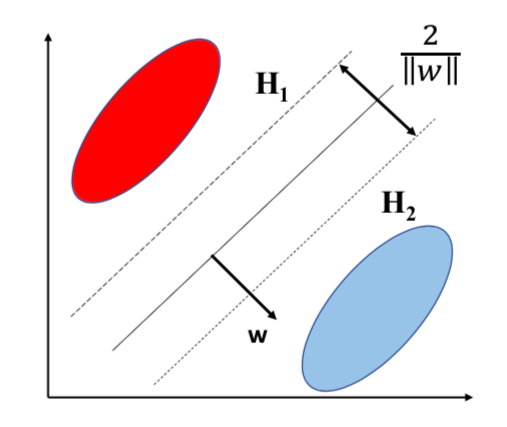
\includegraphics[width=3.0in]{./figures/margin.png}   
	\caption{margin}
	\label{margin}
\end{figure}

\begin{comment}
A very common choice of metric $d$ is the Euclidean metric,
corresponding the $2$-norm $\|\cdot\|_2$. In this case the dual norm
$\|\cdot\|$ is the same. Another reasonable choice could be the
$p$-norm $\|\cdot\|_p$, for $1\leq p\leq \infty$, on $\mathbb{R}^n$.
In this case the dual norm becomes $\|\cdot\|_{p^*}$ where $p^{-1} +
(p^*)^{-1} = 1$.
\end{comment}

\subsection{2-class soft-margin case}

Of course, the following question arises: What should we do if the data is not linearly separable? A possible approach here is to 
replace the hard constraint (\ref{separation_condition_2}) by a penalty term. This is often called a soft-margin SVM,
as opposed to the hard constraint, which is called a hard-margin SVM.

A common choice of penalty is the hinge, or ReLU penalty, which only penalizes when each of the constraints
in (\ref{separation_condition_2}) is violated. The resulting optimization problem takes the following form:
\begin{equation}
 \min_{W,~b} \|w_1-w_2\| + C\displaystyle\sum_{i=1}^N \text{RuLU}\Big(\|y_i - e_j\|_1- (y_i - e_j)\cdot (Wx_i+b) \Big)
\end{equation}
where $C$ is a parameter controlling how much the penalty term is weighted.
